\documentclass[12pt]{article}
\usepackage{amsmath}
\usepackage{mathtools}
\usepackage{tikz}

\begin{document}

\begin{center}
\large\bf University of Waterloo\\
CS~466 --- Advanced Algorithm\\
Spring 2013\\
Problem Set 3\\
Siwei Yang - 20258568\\
\end{center}
\bigskip

\begin{enumerate}

\item{} [8 marks: Using Doubling Binary Search]
This question finishes up the proof that the approximation to the optimal binary search tree can be found in linear time if the probabilities of access to keys (and for unsuccessful searches for values between consecutive key values) are given in order by the key values. Having made this introduction we pose the problem in a straightforward mathematical form.

\begin{itemize}

\item[a.]{[3 marks]}
State the recurrence for the time, T(n), for the algorithm outlined
below:

\begin{itemize}
\item[-] You take time $\lg{i}$ to break a problem of size n into 2 subproblems of sizes i-1
and n-i.
\item[-] You have no control over i, other than it is an integer in the range [1,$\frac{n}{2}$].
\item[-] Problems of size 0 and 1 take no time.
\end{itemize}

We can conclude the recurrence series of this algorithm as:
\begin{equation}
T(n) = 
\begin{dcases}
   T(i-1) + \lg{i} + T(n-i),          & \text{if } n \geq 2\\
    0,                                        & \text{otherwise}
\end{dcases}
\end{equation}

\item[b.]{[5 marks]}
Show that the solution to the recurrence (and so runtime of the algorithm) above is O(n).
below:

Let the base case be:
\begin{equation} \label{eq:base}
T(n) \leq 2 * n - \lg{(n+1)}
\end{equation}
which is true for n = 1.

Then, for the induction step, \textbf{assuming equation~\ref{eq:base} holds for $n < k$}, for a problem of size k, we have:
\begin{equation} \label{eq:ind-1}
T(i-1) + \lg{i} \leq 2 * i
\end{equation}

\begin{equation} \label{eq:ind-2}
T(i-1) + \lg{i} + T{(k-i)} \leq 2 * (k-1) - \lg{(k-i+1)}
\end{equation}

Since we have i in range [1,$\frac{k}{2}$], we have 2 * (k-i+1) > k + 1. Thus, $ \lg{(k+1)} - \lg{(k-i+1)} \leq 1 $. From that fact, part of equation~\ref{eq:ind-2} have this:

\begin{equation} \label{eq:ind-3}
\lg{(k-i+1)} -2 = - \lg{2 * (k-i+1)} - 1 \leq 2 * k - \lg{(k+1)} - 1
\end{equation}

Therefore we can rewrite equation~\ref{eq:ind-2} as:

\begin{equation} \label{eq:ind-3}
T(i-1) + \lg{i} + T{(k-i)} \leq 2 * k - \lg{(k+1)} - 1
\end{equation}

From above, we proved \textbf{equation~\ref{eq:base} holds for $n \leq k$}. Since the base case is true for n = 1, \textbf{we have equation~\ref{eq:base} true for all positive n which means T(n) is in O(n)}.

\end{itemize}

\medskip

\item{} [4 marks: Near-optimal Binary Search Tree]
This question also deals with the “approximately optimal” binary search tree heuristic. The method we discussed works as follows.

\begin{itemize}
\item[-] Choose the root by a greedy heuristic and recursively solve the problem for the left and right subtrees.
\item[-] The root chosen has the key value such that the maximum of the probability of being in its left subtree and the probability of being in its right subtree is minimized.
\end{itemize}

Consider ther following probability distribution:
\begin{center}
\begin{tabular}{l*{8}{c}r}
Interval          & q0 & p1 & q1 & p2 & q2 & p3 & q3                     \\
\hline
Probability       & 0 & 0.49 & 0 & 0.02 & 0 & 0.49 & 0                   \\
\end{tabular}
\end{center}

following the heuristic we have a tree like this:
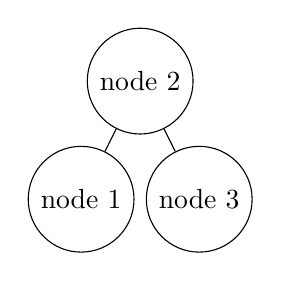
\begin{tikzpicture}
\node[circle,draw](z){node 2}
  child{
node[circle,draw]{node 1} child[missing] child[missing]
  }
  child{
node[circle,draw]{node 3} child[missing] child[missing]
  };
\end{tikzpicture}
the amortized cost for accessing this tree is $2 * 0.49 + 0.02 + 2 * 0.49 = 1.98$.

However, the optimal search tree have the following form:
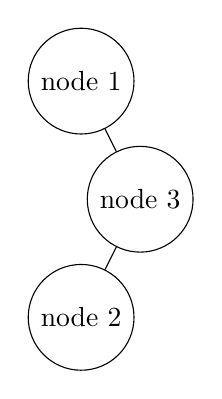
\begin{tikzpicture}
\node[circle,draw](z){node 1}
  child[missing]
  child{
node[circle,draw]{node 3} child{node[circle,draw] {node 2}} child[missing]
  };
\end{tikzpicture}
the amortized cost for accessing this tree is $0.49 + 3 * 0.02 + 2 * 0.49 = 1.53$.


\end{enumerate}

\end{document}

